\documentclass{article}
\usepackage[utf8]{inputenc}
\usepackage{algorithm}
\usepackage{algorithmic}
\usepackage{graphicx} % more modern
\usepackage{subfigure} 
\usepackage{times}
\usepackage{helvet}
\usepackage{courier}
\usepackage{numberedblock}
\setlength\blockindent{0.0in}
\usepackage{hyperref}

\hypersetup{
    colorlinks=true,
    linkcolor=blue,
    filecolor=magenta,      
    urlcolor=cyan,
}

\title{Use NLTK to Write Your Own Sherlock Novel}
\author{Cat McQueen}

\begin{document}

\maketitle

\section{Get Started on Google Colab}
Google Colab is an environment that allows you to do Machine and Deep Learning for free. It can be connected to GitHub and has GPUs that you can use for free. It runs as a Jupyter notebook.

Google Colab is found at https://colab.research.google.com and requires a gmail account. Sign into your gmail account and it will open a pop-up. 
In the bottom right corner, select "NEW NOTEBOOK".

The window should appear the same as Figure~\ref{fig:home}

\begin{figure}[h!]
\centering
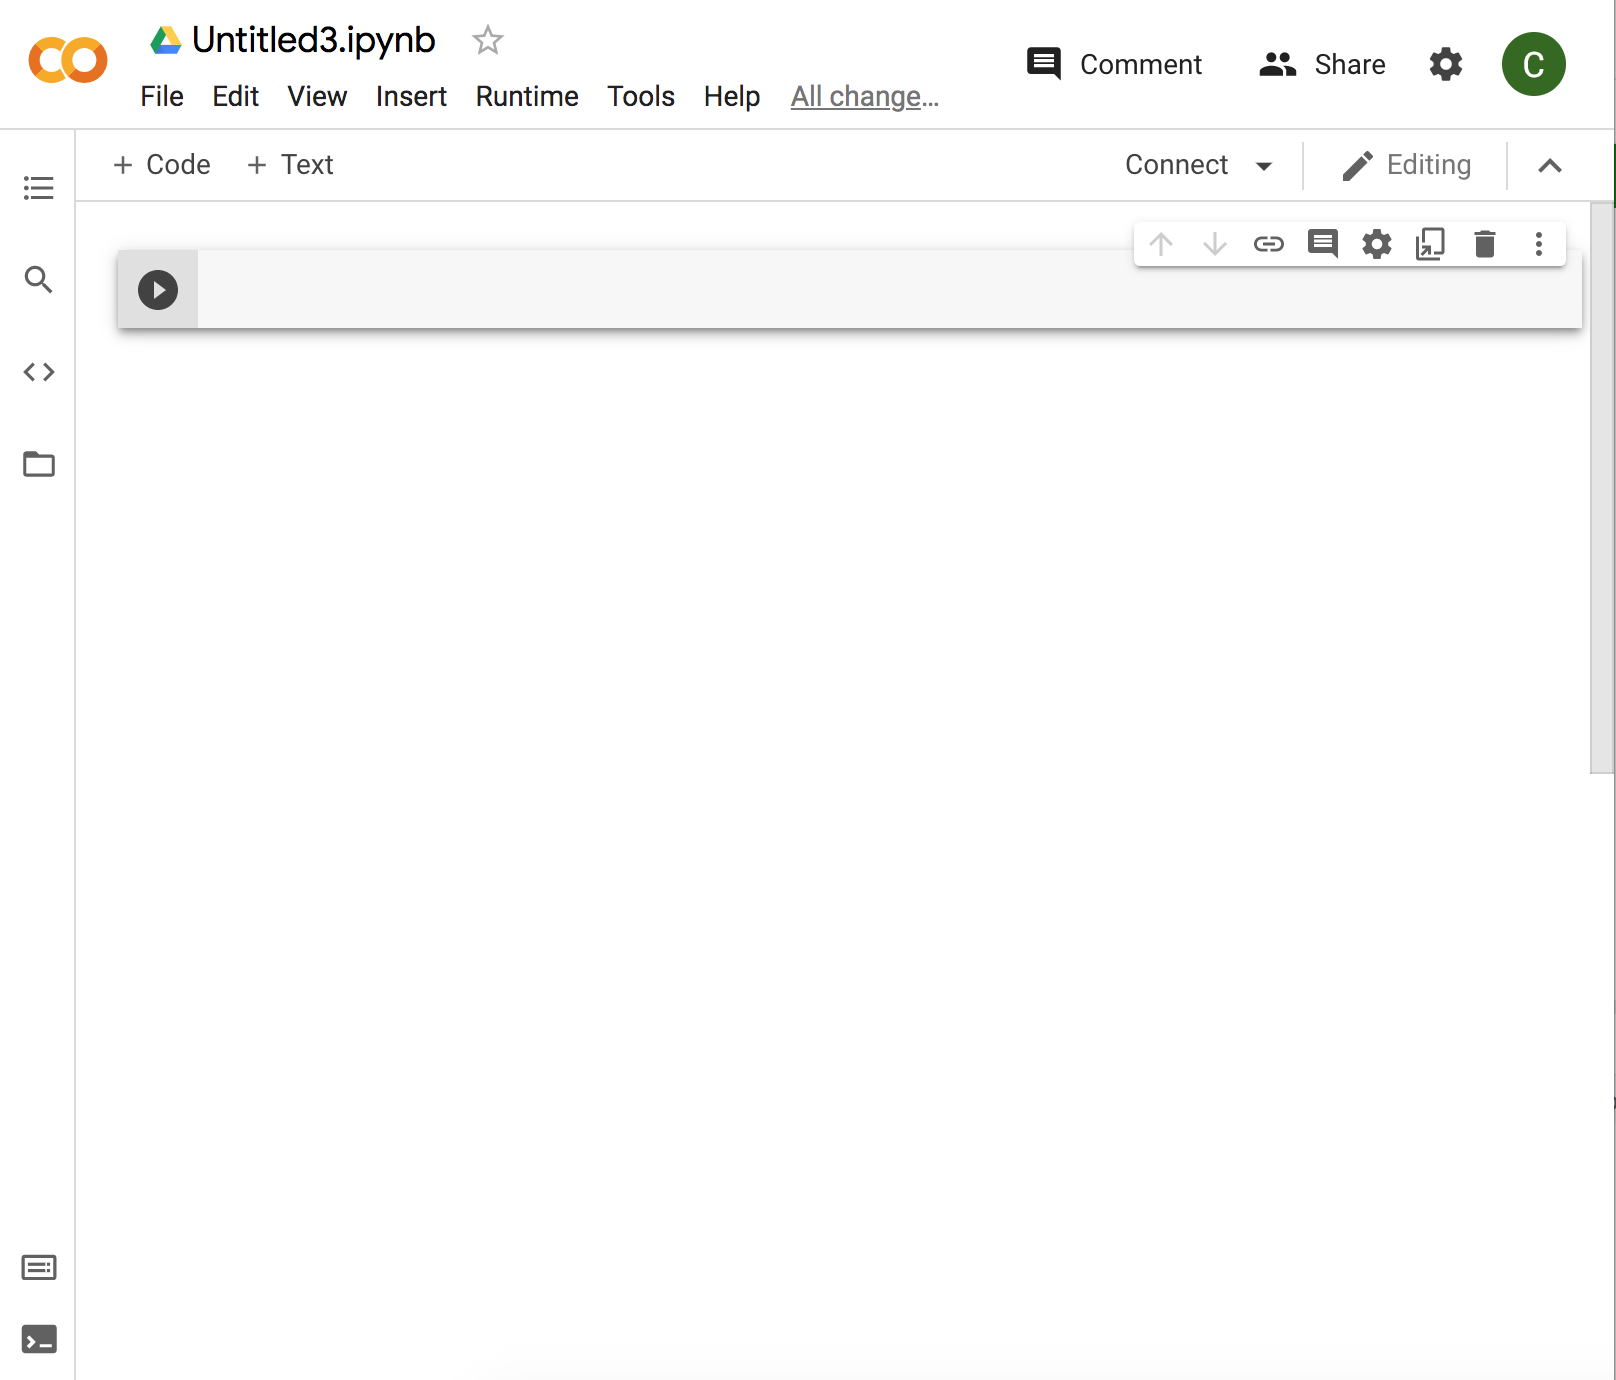
\includegraphics[width=50mm]{ColabHome.png}
\caption{Colab Homepage}
\label{fig:home}
\end{figure}

Now that we're on the right location, we can start coding!

\section{Import data}
The first thing we are going to do is import our Sherlock text file. Sherlock Holmes written by Conan Doyle is now in the public domain and is a dataset we can use to train. This is important to note: you cannot train networks for public consumption on texts that are currently copyrighted.

\textbf{Method 1 (Temporary Upload):} 

To download for this session only (the session will time out after some period of inactivity on the page).

First, download the data onto your local system by downloading 
\href{https://github.com/CatMcQueen/catmcqueen.github.io/blob/b67a282c9be6bfd1ed17796c2507b9108cffb6bc/sherlock.txt}{the Sherlock Text}. On the webpage, on the right, there is a Download button that will allow you to download this text.

Then, we are going to import it into our local Colab you have started. On the side of your colab noteboook, you will see a file icon (the fourth icon down on the left bar), if you click on it you will see a folder location. In order to connect to the folder location, you need to be connected to the runtime, which requires you run something. To get the file folder connected, type
\begin{verbatim}
    print('hello world')
\end{verbatim} 
Then while still inside the text box, press shift and Enter. This will run the code within the box you are currently in.

Repeat every new Run time:
You will then see an empty folder path. We are going to upload sherlock.txt to our setup so we can call it in our python script.

\begin{figure}[h!]
\centering
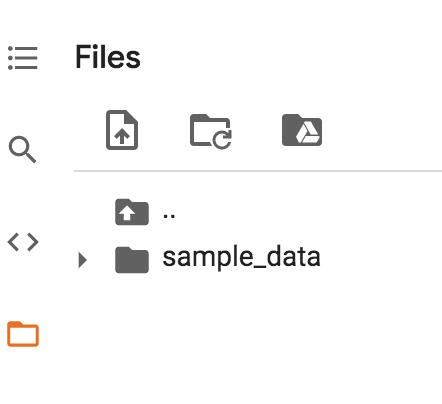
\includegraphics[width=50mm]{FileFolder.png}
\caption{The File Upload Bar}
\label{fig:filefolder}
\end{figure}

Click on the upload icon, and upload the sherlock.txt you previously downloaded to your local system. Now we're ready to read it in and parse the data.

\begin{figure}[h!]
\centering
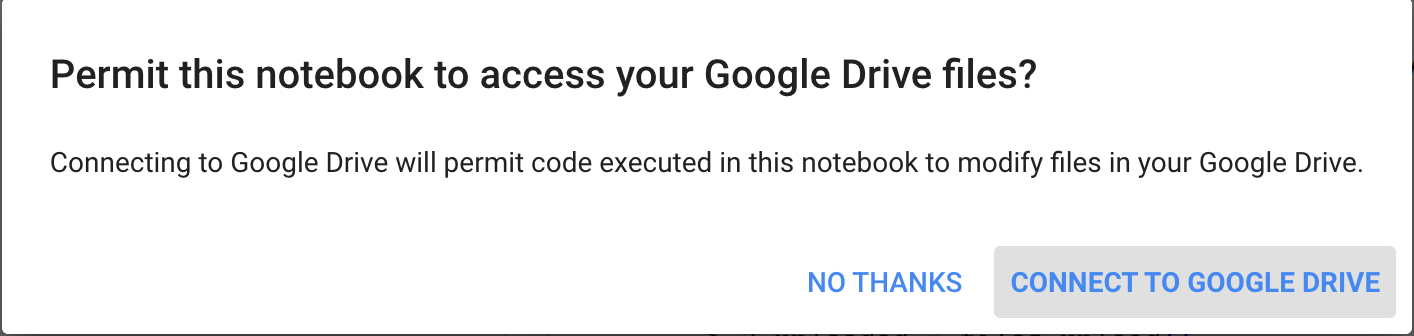
\includegraphics[width=50mm]{GoogleDriveConnect.png}
\caption{Select Connect to Google Drive}
\label{fig:connectdrive}
\end{figure}

\textbf{Method 2 Google Drive:}

First, download the data onto your local system by downloading 
\href{https://github.com/CatMcQueen/catmcqueen.github.io/blob/b67a282c9be6bfd1ed17796c2507b9108cffb6bc/sherlock.txt}{the Sherlock Text}. On the webpage, on the right, there is a Download button that will allow you to download this text.

To upload so the file can be read indefinitely, we'll mount our google drive inline and upload the file from there. First, click on the right Google Drive icon on the file upload page shown in Figure~\ref{fig:filefolder}. You will then see a window pop up asking you to permit it to access your Drive. It may require you to register using an access code the first time. When you see Figure~\ref{fig:connectdrive} pop up, select Connect to Google Drive. Run

\begin{verbatim}
    %cd drive/My Drive/
\end{verbatim}

If you have saved sherlock.txt within another folder in Google Drive, append the folder path to the path in the cd command. We will now be able to run our script even after the runtime disconnects without loading sherlock.txt again.

\textbf{Method 3 (Recommended):}
We are going to do a git checkout from this repository of just the sherlock.txt. This link can be found by going to \href{https://github.com/CatMcQueen/catmcqueen.github.io/blob/main/sherlock.txt}{the Sherlock Text} and copying the permalink from that webpage.

\begin{verbatim}
    ! wget https://github.com/CatMcQueen/
    catmcqueen.github.io/blob/
    69193fa4c4914f40aa57c58476018a13c3258435/sherlock.txt
\end{verbatim}

This will import sherlock.txt to the local runtime and allow it to be called.

\section{Read and Process File}
The first thing we are going to do is to read the text file in. Now that we have the sherlock.txt in our local runtime, read the file into a variable. Remember to close the file after loading the data.

\begin{verbatim}
# Open a file: sherlock.txt in read mode
file = open('sherlock.txt',mode='r')
 
# read all lines into sherlock_txt
sherlock_txt = file.read()
 
# close the file
file.close()
\end{verbatim}

Now that you have the file, we are going to process it. This entails
1) removing punctuation and numbers, 2) removing any unnecessary white space, 3) reformatting into sentences, instead of lines. Once the data is processed, we can tokenize it and begin to use the data.

\textbf{1: Removing Digits and White Space}
Remove all empty lines:
While sherlock.txt does have all empty lines removed already, this will cover any new document that does not have the empty lines removed
\begin{verbatim}
    filter(None, sherlock_txt)
\end{verbatim}
This line will remove all lines that are ['']. These are the ones that are an empty line in the text. We don't want to learn whitespaces, so we'll remove them here. 

To remove digits we are going to use regular expressions. the regular expression for removing numbers is \begin{verbatim} re.sub('[0-9]*', ' ')
\end{verbatim}
Generally, re.sub('x','y') means to replace all x with y. In this case the x is \begin{verbatim}
    \[0-9]*
\end{verbatim}
[0-9] represents all numbers from 0-9. Adding the *, means that any pattern of numbers (greater or equal to 0 digits in a sequence), will be replaced by y, which in this case is ' ', meaning that we are replacing all sequences of numbers of any size with a space. 


Next we'll remove all tabs and other forms of white space and replace them with spaces. In the same fashion as before, we'll use re.sub.
\begin{verbatim}
    re.sub(r'\s+', ' ')
\end{verbatim}
 In this case, r' means to not use the backslash as a literal character, but to use it as part of the spaces. 
 \begin{verbatim}
    '\s+'
 \end{verbatim}
 represents all whitespaces, so we are replacing all white spaces with a single space.
 
\end{document}

